\documentclass[oneside, 11pt]{article}

\usepackage[T1]{fontenc}
\usepackage[utf8]{inputenc}
\usepackage[dutch]{babel}

\usepackage{fouriernc}
\usepackage[detect-all, load-configurations=binary,
            separate-uncertainty=true, per-mode=symbol,
            retain-explicit-plus, range-phrase={ tot }]{siunitx}

\usepackage{setspace}
\setstretch{1.2}

\setlength{\parskip}{\smallskipamount}
\setlength{\parindent}{0pt}

\usepackage{geometry}
\geometry{marginparwidth=0.5cm, verbose, a4paper, tmargin=3cm, bmargin=3cm, lmargin=2cm, rmargin=2cm}

\usepackage{float}

\usepackage[fleqn]{amsmath}
\numberwithin{equation}{section}
\numberwithin{figure}{section}

\usepackage{graphicx}
\graphicspath{{Figures/}}
\usepackage{subfig}

\usepackage{tikz}
\usetikzlibrary{plotmarks}

\usepackage{fancyhdr}
\pagestyle{fancy}
\fancyhf{}
\rhead{\thepage}
\renewcommand{\footrulewidth}{0pt}
\renewcommand{\headrulewidth}{0pt}

\usepackage{relsize}
\usepackage{xspace}
\usepackage{url}

\newcommand{\figref}[1]{Figuur~\ref{#1}}

\newcommand{\hisparc}{\textsmaller{HiSPARC}\xspace}
\newcommand{\kascade}{\textsmaller{KASCADE}\xspace}
\newcommand{\sapphire}{\textsmaller{SAPPHiRE}\xspace}
\newcommand{\jsparc}{\textsmaller{jSparc}\xspace}
\newcommand{\hdf}{\textsmaller{HDF5}\xspace}
\newcommand{\aires}{\textsmaller{AIRES}\xspace}
\newcommand{\csv}{\textsmaller{CSV}\xspace}
\newcommand{\python}{\textsmaller{PYTHON}\xspace}
\newcommand{\corsika}{\textsmaller{CORSIKA}\xspace}
\newcommand{\labview}{\textsmaller{LabVIEW}\xspace}
\newcommand{\daq}{\textsmaller{DAQ}\xspace}
\newcommand{\adc}{\textsmaller{ADC}\xspace}
\newcommand{\adcs}{\textsmaller{ADC}s\xspace}
\newcommand{\Adcs}{A\textsmaller{DC}s\xspace}
\newcommand{\hi}{\textsc{h i}\xspace}
\newcommand{\hii}{\textsc{h ii}\xspace}
\newcommand{\mip}{\textsmaller{MIP}\xspace}
\newcommand{\hisparcii}{\textsmaller{HiSPARC II}\xspace}
\newcommand{\hisparciii}{\textsmaller{HiSPARC III}\xspace}
\newcommand{\pmt}{\textsmaller{PMT}\xspace}
\newcommand{\pmts}{\textsmaller{PMT}s\xspace}

\DeclareSIUnit{\electronvolt}{\ensuremath{\mathrm{e\!\!\:V}}}

\DeclareSIUnit{\unitsigma}{\ensuremath{\sigma}}
\DeclareSIUnit{\mip}{\textsmaller{MIP}}
\DeclareSIUnit{\adc}{\textsmaller{ADC}}

\DeclareSIUnit{\gauss}{G}
\DeclareSIUnit{\parsec}{pc}
\DeclareSIUnit{\year}{yr}




\title{Achtergrondinformatie Stationsonderhoud}
\author{C.G.N. van Veen}
\docwerkblad{1}{LSO}
\version{1.0}

\begin{document}

\maketitle

\section{Les 1. Kosmische straling}

De aarde wordt continu `gebombardeerd' door deeltjes vanuit de ruimte.
Als zo'n deeltje de dampkring binnendringt zal het op een gegeven moment
een botsing maken met een luchtmolecuul. Met `botsing' bedoelen we niet
een botsing zoals tussen biljartballen. Bij een botsing tussen
biljartballen verandert wel de richting en snelheid van de
biljartballen, maar er ontstaan geen nieuwe biljartballen. Het is beter
te spreken van een \emph{wisselwerking} tussen het kosmisch deeltje en
een luchtmolecuul omdat tijdens de wisselwerking nieuwe deeltjes
ontstaan. Deze deeltjes zullen op hun beurt ook weer wisselwerken met
luchtmoleculen waardoor er nog meer nieuwe deeltjes ontstaan. Er
ontstaat als het ware een `lawine' van deeltjes, die in de
wetenschappelijke literatuur wordt aangeduid als \emph{cosmic air
shower}. Bij elke wisselwerking wordt de energie verdeeld over de nieuwe
deeltjes waardoor de energie per deeltje afneemt. Deeltjes waarvan de
energie te klein is om bij een wisselwerking nieuwe deeltjes te maken
dragen niet meer bij aan de ontwikkeling van de lawine; de lawine
`sterft uit'. Hoe groter de energie van het deeltje dat uit de ruimte
kwam, des te langer het duurt voor dat de lawine is uitgestorven. Als de
energie groot genoeg is kan de lawine het aardoppervlak bereiken. 
verder weg uit de ruimte komen deeltjes met hogere energie. Van de
lawines die daaruit in onze atmosfeer ontstaan kunnen deeltjes het
aardoppervlak bereiken en een signaal afgeven in een \hisparc detector.
Op deze wijze kunnen we kosmische deeltjes indirect waarnemen. In deze
lesbrief zal worden ingegaan op de ontwikkeling van de shower in de
atmosfeer en de deeltjes die daarbij een belangrijke rol spelen. 
Kosmische deeltjes kunnen een relatief hoge energie hebben, tot wel meer
dan \SI{e20}{\electronvolt}. De energie van energetische deeltjes wordt
vaak uitgedrukt in \SI{}{\tera\electronvolt}, \SI{}{\peta\electronvolt},
etc.

\subsection{Elektromagnetische showers}

Wanneer een kosmisch gamma-deeltje $\gamma$ (een hoogenergetisch foton)
de dampkring binnenkomt, kan het door elektromagnetische wisselwerking
met de kern van een luchtatoom opsplisten in een elektron $e^-$ en een
positron $e^+$. Dit proces heet paar-creatie. Wat verderop in de
dampkring kan het elektron vervolgens door elektromagnetische
wisselwerking met de kern van een luchtatoom een gamma-deeltje afstaan.
Hetzelfde geldt voor het positron. Dit proces heet remstraling. Weer wat
verderop in de dampkring zal er weer paar-creatie optreden bij de
gamma-deeltjes en remstraling bij de elektronen en positronen. Er komen
dus steeds meer deeltjes, maar die hebben elk wel een steeds kleinere
energie. Na een aantal splitsingen is de energie van een deeltje zo
klein dat het gemakkelijk zijn energie kwijtraakt aan het ioniseren van
een luchtatoom. Dat gebeurt als de energie van een deeltje nog maar zo'n
\SI{84}{\mega\electronvolt} is. Voordat het zover is kunnen er uit één
kosmisch deeltje een lawine van vele miljoenen deeltjes in de dampkring
ontstaan: de \emph{cosmic air shower} of kortweg \emph{shower}. Omdat
zowel paar-creatie als remstraling elektromagnetische processen zijn
spreekt men van een elektromagnetische shower. \\

Samenvattend wordt de elektromagnetische shower gedomineerd door paar-creatie
\begin{equation}
    \gamma \rightarrow e^- + e^+ \nonumber
\end{equation}
en remstraling
\begin{equation} 
    e^\pm \rightarrow e^\pm + \gamma \ . \nonumber
\end{equation}
In beide gevallen is er een `splitsing' van één deeltje in twee deeltjes.  

\subsection{Hadronische showers}

Wanneer een kosmisch proton $p$ de dampkring binnenkomt, kan het een
sterke (hadronische) wisselwerking aangaan met de kern van een
luchtatoom. Het gevolg is dat er een groot aantal pionen ontstaat.
Daarvan is ongeveer een derde deel positief geladen ($\pi^+$), een
derde deel negatief geladen ($\pi^-$) en  een derde deel ongeladen
(neutraal) ($\pi^0$). De neutrale pionen hebben een extreem korte
levensduur; ongeveer \SI{8,4e-17}{\second} in rust. Ze vervallen daardoor
direct in twee gamma-deeltjes die elk een elektromagnetische shower
teweegbrengen zoals hiervoor beschreven. De geladen pionen hebben een
langere levensduur; ongeveer \SI{2,6e-8}{\second} in rust. De hoge snelheid
van de geladen pionen veroorzaakt tijddilatatie (een gevolg van de
relativiteitstheorie) waardoor de levensduur veel groter is. Het gevolg
is dat de geladen pionen een sterke wisselwerking aangaan met de kern
van een luchtatoom voor dat hun levensduur voorbij is. Daarbij ontstaan
weer nieuwe pionen, waarvan weer een derde deel $\pi^+$, een derde
deel $\pi^-$ en een derde $\pi^0$. De neutrale pionen daarvan
vervallen weer direct tot twee gamma deeeltjes, terwijl de geladen
pionen weer een sterke wisselwerking aan kunnen gaan, enzovoort. Na een
aantal sterke wisselwerkingen is de energie van per pion, en daarmee ook
zijn levensduur, zodanig afgenomen dat het pion vervalt voordat het een
sterke wisselwerking aangaat. Het geladen pion vervalt dan in een muon
$\mu$ (met dezelfde lading als het pion) en een muonneutrino $\nu_\mu$
(ongeladen). In een schema:
\begin{equation}
    \pi^+ \rightarrow \mu^+ + \nu_\mu \ , \nonumber
\end{equation}
\begin{equation}
    \pi^- \rightarrow \mu^- + \bar{\nu}_\mu \ , \nonumber
\end{equation}
\begin{equation}  
    \pi^0 \rightarrow \gamma + \gamma \ . \nonumber
\end{equation}

Net als de pionen hebben de muonen ook een eindige levensduur; ongeveer
$2,2 \cdot 10^{-6}$ s in rust. De muonen die in de hadronische shower
ontstaan hebben een dusdanige hoge energie (en daarmee een dusdanige
levensduur) dat ze veelal het aardoppervlak bereiken. Omdat ze geladen
zijn kunnen ze net als de elektronen een signaal afgeven in de \hisparc
detector. De muonen die niet het aardoppervlak bereiken zijn ergens in
de lucht vervallen in een elektron en twee verschillende neutrino's:
\begin{equation}
    \mu^+ \rightarrow e^+ + \nu_e + \bar{\nu}_\mu \ , \nonumber
\end{equation}
\begin{equation}
    \mu^- \rightarrow e^- + \bar{\nu}_e + \nu_\mu \ . \nonumber
\end{equation}  

Sommige elektronen (positronen) die ontstaan zijn uit het verval van
muonen kunnen alsnog het aardoppervlak bereiken en een signaal afgeven
in een \hisparc detector.
\\

De hadronische shower is belangrijk omdat bijna 90\% van de kosmische
deeltjes protonen zijn.

\subsection{Deeltjes meten}

De \hisparc stations meten de deeltjes van de shower die
het aardoppervlak bereiken en zijn via een netwerk verbonden met het
Nikhef en de Universiteit van Nijmegen. De \hisparc detectoren kunnen
de fotonen, muonen en elektronen meten die in zo’n shower voorkomen.
Een station bestaat uit twee of vier detectoren, die ieder
een eigen signaal bij een detectie van een EAS geven; de pulshoogte. Is
het signaal hoog genoeg en meten twee of meer detectoren binnen een kort
tijdspanne een signaal, dan slaat het meetstation dit signaal als een
event op in de database. Het registreren van een signaal in een detector wordt 
uitgebreid uitgelegd in het document "Inregelen PMT's". 
Per uur worden typisch zo’n 2000 tot 3000
events geregistreerd per station. Als meerdere detectoren of stations
binnen een bepaalde tijd deeltjes detecteren dan spreken we van een
coïncidentie. Bij een coïncidentie behoren dus alle metingen op dat
moment bij één shower.

In \figref{fig:pulshoogte} zie je de pulsen van twee detectoren (dit is
dus een twee detector station of een vier detector station, waarbij twee 
detectoren `getriggerd' zijn). De maximale waarde van de pulsen is daar
aangegeven met een verticale lijn. De waarde van de potentiaal die bij
dit punt hoort, wordt de `pulseheight' of in het Nederlands `pulshoogte'
genoemd. Als we van alle events, die we op een dag meten met een
station, alle gemeten `pulseheights' plotten in een histogram dan
krijgen we het plaatje zoals te zien is in \figref{fig:MIP_histogram}. Daarin
zetten we het aantal keer dat een bepaalde pulshoogte voorkomt uit tegen
de spanningswaarde van de pulshoogte. De laagste piek van de pulshoogte
komt het vaakst voor en deze waarde geeft dus een maat voor de detectie van
precies één deeltje in een detector. Stel dus dat de waarde van de
pulshoogte -180 mV heel vaak voorkomt op een dag. Dan zul je in het
pulshoogte histogram een piek krijgen bij 180 mV (we nemen nu het
potentiaalverschil positief), dit is dan de waarde die hoort bij één
deeltje wat gedetecteerd is. Meet je bij een ander event in een detector
een puls van -540 mV, dan zouden er 3 deeltjes zijn gedetecteerd
zijn door deze detector. De piek in het pulshoogte histogram noemen we
de MIP (Minimum Ionizing Particle) dat is waarde van de rode lijn in
\figref{fig:MIP_histogram} (in dit geval ongeveer 180 mV).

\begin{figure}
    \centering
    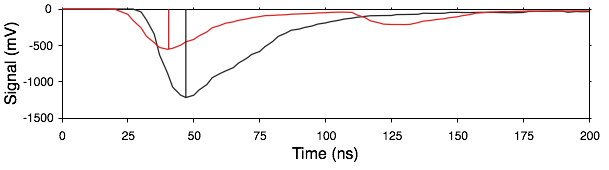
\includegraphics[scale=0.8]{pulshoogte}
    \caption{Pulseheights van twee detectoren aangegeven.}
    \label{fig:pulshoogte}
\end{figure} 

\begin{figure}
    \centering
    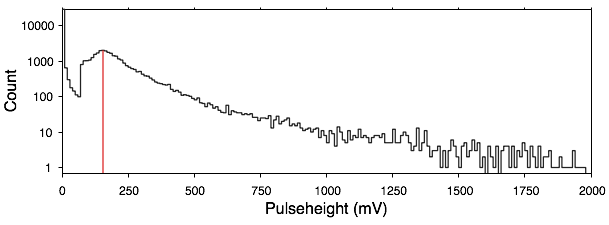
\includegraphics[scale=0.8]{MIP_histogram}
    \caption{Een pulshoogte histogram, in dit diagram zijn de pulseheights van veel 
    gemeten events door één detector uitgezet. De piek is de pulshoogte,
    die hoort bij de detectie van één deeltje. Dit is de MIP piek. In dit geval is
    de MIP +/- 180 mV. De MIP piek wordt gebruikt om de deeltjes
    dichtheid in de detector voor alle geregistreerde events uit te
    rekenen.}
    \label{fig:MIP_histogram}
\end{figure} 

Nu we met behulp van de MIP\footnote{Meer over de MIP piek vind je in
het bestand `inregelen PMT's' van het \hisparc infopakket} piek van elke
detector kunnen bepalen wat het aantal deeltjes in een detector per
event is. Als het aantal deeltjes per detector bekend is kunnen we de
energie van het primaire deeltje wat de shower veroorzaakt
reconstrueren. Omdat we denken te weten hoe de shower zich ontwikkelt in de
atmosfeer, kunnen we met onze metingen van het aantal deeltjes op de
grond aan de hand van een wiskundige vergelijking\footnote{Meer over deze formule in infopakket
`Uitleg \hisparc'} een energie van het primaire deeltje reconstrueren.

\section{Les 2. meetstations van \hisparc}

Zodra een shower een detector bereikt gaan één of meerdere deeltjes
door de detector.  Dit veroorzaakt een pulsvormig signaal (\figref{fig:pulshoogte}).
De relatief lange staart van het signaal wordt veroorzaakt door licht dat via een
aantal reflecties alsnog bij de \pmt terecht komt, maar ook door deeltjes
die een beetje achterliepen in de shower en vrij laat door de detector
gaan.  Het signaal uit de \pmt wordt via kabels met een lengte van
\SI{30}{\meter} naar de \hisparc elektronica geleid.  Alle kabels zijn
precies even lang, om te zorgen dat het signaal uit alle detectoren op
hetzelfde moment bij de elektronica aankomt.

